\documentclass[12pt, titlepage]{article}

\usepackage{booktabs}
\usepackage{tabularx}
\usepackage{hyperref}
\usepackage{graphicx}
\usepackage[normalem]{ulem}
\usepackage{xcolor}
\graphicspath{ {./} }
\hypersetup{
    colorlinks,
    citecolor=black,
    filecolor=black,
    linkcolor=red,
    urlcolor=blue
}
\usepackage[round]{natbib}

\title{SE 3XA3: Software Requirements Specification\\BlockBuilder}

\author{Team 28, OAC
		\\ Owen McNeil, mcneilo
		\\ Christopher DiBussolo, dibussoc
		\\ Andrew Lucentini, lucenta
}

\date{\today}

%\input{../Comments}

\begin{document}

\maketitle

\pagenumbering{roman}
\tableofcontents
\listoftables
\listoffigures

\begin{table}[bp]
\caption{\bf Revision History}
\begin{tabularx}{\textwidth}{p{3cm}p{2cm}X}
\toprule {\bf Date} & {\bf Version} & {\bf Notes}\\
\midrule
Oct 5, 2018 & 1.0 & Initial creation of the SRS pushed to repo\\
\midrule
\textcolor{red}{Dec 1, 2018} & \textcolor{red}{2.0} & \textcolor{red}{Begin making changes for rev1}\\
\midrule
\textcolor{red}{Dec 5, 2018} & \textcolor{red}{2.1} & \textcolor{red}{Final changes made for rev1}\\
\bottomrule
\end{tabularx}
\end{table}

\newpage

\pagenumbering{arabic}

This document describes the requirements for BlockBuilder. The template for the Software
Requirements Specification (SRS) is a subset of the Volere
template~\citep{RobertsonAndRobertson2012}.

\section{Project Drivers}

\subsection{The Purpose of the Project}
The purpose of this project is to provide people a fun and free open world video game for people to unleash their creativity.
\subsection{The Stakeholders}

\subsubsection{The Client}
\sout{The clients of BlockBuilder are potential users of all age above 4 years who will play the game itself. The users must be satisfied with the product upon delivery.}
\textcolor{red}{The client for the BlockBuilder project is the 3XA3 professor, Dr. Asghar Bokhari.}
\subsubsection{The Customers}
In this situation, the customers are the same as the client. The customers of this product are individuals of all age above 4 years who own a personal or desktop computer. Since BlockBuilder will be free, anyone has the ability to download the game and use it in their own time.
\subsubsection{Other Stakeholders}
Additional stakeholders of the product include the following:
\begin{itemize}
\item \sout{The TA's of SE3XA3}
\item \textcolor{red}{The devlopement team, consisting of Owen McNeil, Chris DiBussolo and Andrew Lucentini}
\item \sout{The professor of SE3XA3}
\end{itemize}
\subsection{Mandated Constraints}
This section describes the constraints on the eventual design of the software.
\subsubsection{Solution Constraints}

\textbf{Description}: The product shall operate using a Windows OS (ideally Windows 7 or higher) and/or MacOSX.\\
\textbf{Rationale}: The average user utilizes either one of these operating systems.\\
\textbf{Fit criterion}: The product shall be approved on both Mac and Windows operating systems.
\subsubsection{Implementation Environment of the Current System}

\textcolor{red}{N/A}

\subsubsection{Partner or Collaborative Applications}

The software shall run with the Pyglet library for graphic generation. The software will not run correctly if the Pyglet package is not installed on the user's computer.

\subsubsection{Off-the-Shelf Software}

\textbf{Description}: The product shall utilize the Pyglet library for 3D graphics support.\\
\textbf{Rationale}: Development costs and development time will be greatly reduced. Performance will likely be better than developing an engine in-house.\\
\textbf{Fit criterion}: The product will be built on top of Pyglet and integration tests will be performed.

\subsubsection{Anticipated Workplace Environment}
\textbf{N/A}
\subsubsection{Schedule Constraints}

\begin{itemize}
    \item The documentation of the software shall be delivered by each deadline provided by the SE3XA3 outline.
    \item The final implementation of BlockBuilder shall be complete by December 5, 2018.
\end{itemize}

\subsubsection{Budget Constraints}
\textbf{N/A}

\subsection{Naming Conventions and Terminology}
\textbf{FPS} - Frames per second. A measurement for how many unique consecutive images a monitor can handle each second.\\
\textbf{GUI} - Graphical user interface. It includes graphical elements, such as windows, icons and buttons.\\
\textcolor{red}{\textbf{3D} - Rendering on a 3-dimensional plane consisting of (x,y,z) coordinates.}\\
\textcolor{red}{\textbf{Minecraft} - 3D first-person sandbox game developed by Mojang.}\\
\textcolor{red}{\textbf{Pyglet} - Python multimedia library used for 2D and 3D graphics rendering.}\\

\subsection{Relevant Facts and Assumptions}

\subsubsection{Relevant Facts}

\begin{itemize}
    \item Pyglet has been proven to be capable of effectively powering a 'Minecraft' style 3D game.
    \item The original project has approximately 900 lines of code.
\end{itemize}

\subsubsection{Relevant Assumptions}

The target user of this product is assumed to be:
\begin{itemize}
    \item Physically and mentally capable of enjoying a video game.
    \item Interested in open-world video games.
    \item Accepting of "blocky" and low-resolution style graphics.
    \item Creative.
\end{itemize}

It is assumed that the average user will have:
\begin{itemize}
    \item A modern computer capable of running a simple 3D Python game.
    \item A keyboard and mouse.
    \item \textcolor{red}{The game will also allow the use of a track-pad if being played on a laptop.}
    \item A monitor capable of refreshing at REFRESH\_RATE
\end{itemize}

\section{Functional Requirements}

\subsection{The Scope of the Work and the Product}

\subsubsection{The Context of the Work}

\begin{figure}[!htbp]
  \caption{BlockBuilder Context Diagram}
  \centering
    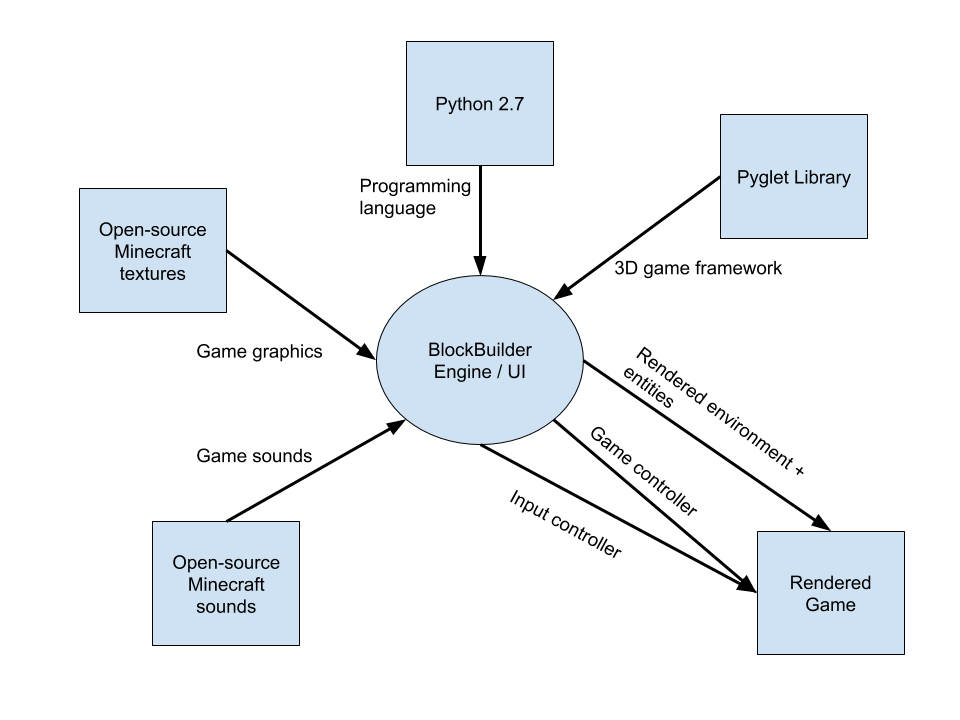
\includegraphics[width=0.8\textwidth]{req_context_diagram}
\end{figure}
\newpage
\subsubsection{Work Partitioning}

\begin{table}[!htbp]
\caption{Work Partitioning}
\begin{tabular}{@{}lll@{}}
\toprule
\textbf{Event Name}       & \textbf{Input and Output} & \textbf{Summary}                                                                                                   \\ \midrule
1. Player performs action & Player action (in)        & \begin{tabular}[c]{@{}l@{}}Parse the action in game controller \\ and modify game state as necessary.\end{tabular} \\
2. Chunk boundary reached & Player coordinates (in)   & \begin{tabular}[c]{@{}l@{}}Generate required chunks and \\ render them.\end{tabular}                               \\
3. New entity generated   & New Entity (in)           & \begin{tabular}[c]{@{}l@{}}Create new entity object, add it to \\ render and controller cycles.\end{tabular}       \\ \bottomrule
\end{tabular}
\end{table}

\subsubsection{Individual Product Use Cases}

The primary use case for this product is to be enjoyed as a game that users play in their free time. Given it's open-world, creative nature, and lack of clear objectives, it isn't possible to determine all possible use cases, or play styles.

\subsection{Functional Requirements}
\begin{itemize}
    \item \sout{REQ1: The game must feature textures similar to those present in 'Minecraft'.}
    \item \sout{REQ2: The player should be able to break and place blocks as done in 'Minecraft'.}
    \item \sout{REQ3: The game environment, including the "biomes", entities and overall input/output should mirror that of 'Minecraft'.}
    \item REQ4: The game must be implemented using a \sout{Python 2.7} \textcolor{red}{Python 3.7}/Pyglet stack.
    \item REQ5: \sout{The game must be three dimensional.} \textcolor{red}{The user must be able to move their character in 3-dimensions.}
    \item \sout{REQ6: The player must be able to control their character.}
    \item \textcolor{red}{REQ6: The user must be able to move their character in the forward direction while the 'W' key is pressed.}
    \item \textcolor{red}{REQ7: The user must be able to move their character in the left direction while the 'A' key is pressed.}
    \item \textcolor{red}{REQ8: The user must be able to move their character in the right direction while the 'D' key is pressed.}
    \item \textcolor{red}{REQ9: The user must be able to move their character in the backward direction while the 'S' key is pressed.}
    \item \textcolor{red}{REQ10: The user must be able look around in the game by moving the mouse or trackpad.}
    \item \textcolor{red}{REQ11: The user must be able to simulate a jump in the world when the space bar is pressed.}
    \item \textcolor{red}{REQ12: The user must be able to enter 'Flying mode' when the 'Tab' key is pressed.}
    \item \textcolor{red}{REQ13: The user must be able to place blocks in the world with a mouse right-click provided they are looking at a previously existing block in the world at a minimum distance.}
    \item \textcolor{red}{REQ14: The user must be able to remove blocks in the world with a mouse left-click provided they are looking at a block at a minimum distance.}
    \item \textcolor{red}{REQ15: The user must be able to place Grass blocks after they hit the '1' num key.}
    \item \textcolor{red}{REQ16: The user must be able to place Brick blocks after they hit the '2' num key.}
    \item \textcolor{red}{REQ17: The user must be able to place Sand blocks after they hit the '3' num key.}
    \item \textcolor{red}{REQ18: The user must be able to place Stone blocks after they hit the '4' num key.}
    \item \textcolor{red}{REQ19: The user must be able to remove all blocks (when possible) except Stone blocks.}
    \item \textcolor{red}{REQ20: The game must be robust in it's ability to handle a large variety of user inputs.}
    \item \textcolor{red}{REQ21: The player should not be able to place blocks in a position that would result in a collision between the player and the newly placed block.}
    \item \textcolor{red}{REQ22: The player should not be able to move through blocks and attempting to should result in a "collision" that makes the player unable to move through the block instead makes it look like they are walking into it.}
\end{itemize}


\section{Non-functional Requirements}

\subsection{Look and Feel Requirements}
The look and feel requirements of the product are listed below.
\begin{itemize}
\item \textcolor{red}{LF1: }The product shall be attractive to users of all age with a direct focus on individuals MAX\_FOCUS\_AGE and younger.\\
\textcolor{red}{Fit Criterion: After 2.5 months after release, a survey shall be administered to users MAX\_FOCUS\_AGE and younger to reveal that 90\% of the users liked the product.}
\item \textcolor{red}{LF2: }The GUI of the product should resemble that of Minecraft.\\
\textcolor{red}{Fit Criterion: After 2 months after release, a survey shall be administered to users to reveal that 98\% of the users thought that the product resembled Minecraft.}
\end{itemize}

\subsection{Usability and Humanity Requirements}
This section is concerned with requirements that make the product usable and acceptable to the users.

\subsubsection{Ease of Use Requirements}
\begin{itemize}
\item \textcolor{red}{UH1: }Users of all ages (MIN\_AGE+) should be able to play the game.\\
\textcolor{red}{Fit Criterion: 95\% of the users from a test group aged MIN\_AGE+ shall be able to play the game on their own after 10 minutes of playing the game.}
\item \textcolor{red}{UH2: }The users shall remember how to use the product after 1 session of playing the game.\\
\textcolor{red}{Fit Criterion: After playing the game once, 90\% of the users from a test group shall correctly answer a set of questions asking which inputs correspond to their respective in-game actions.}
\item \textcolor{red}{UH3: }The product shall make the users want to use it.\\
\textcolor{red}{Fit Criterion: After 2.5 months after release, a questionnaire shall be administered to all users to reveal that 90\% of the users wanted to use the product after their first use.}
\item \textcolor{red}{UH4: }The product shall be playable by users of all languages.\\
\textcolor{red}{Fit Criterion: 100\% of users from a test group consisting of 15 users, each speaking different languages, shall be able to play the game on their own after 10 minutes.}
\item \textcolor{red}{UH5: }The user shall interact with the game through the typical "WASD" keyboard control scheme set up.\\
\textcolor{red}{Fit Criterion: A tester shall play the game to ensure that they move their player using the "WASD" keys.}
\end{itemize}

\subsubsection{ Personalization and Internationalization Requirements}
N/A

\subsubsection{Learning Requirements}
\begin{itemize}
\item \textcolor{red}{UH6: }The users shall be able to learn the product within LEARNING\_TIME minutes of playing.\\
\textcolor{red}{Fit Criterion: A team of 10 users shall perform a test after LEARNING\_TIME minutes to reveal that 95\% of the users can teach the game to another user.}
\item \textcolor{red}{UH7: }The software shall be learnable without a tutorial.\\
\textcolor{red}{Fit Criterion: A team of 20 users shall perform a test after LEARNING\_TIME minutes to reveal that 98\% of the users can play the game without instructions.}
\item \textcolor{red}{UH8: }The software shall be learnable by any user above the age of MIN\_AGE regardless of educational background.\\
\textcolor{red}{Fit Criterion: A team of 15 users with various educational backgrounds (including none) shall perform a test after LEARNING\_TIME minutes to reveal that 98\% of the users can play the game without instructions.}
\end{itemize}

\subsubsection{Understandability and Politeness Requirements}
\begin{itemize}
\item \textcolor{red}{UH9: }The software shall not use any complicated text that may confuse the user.\\
\textcolor{red}{Fit Criterion: After 2 weeks upon release, a questionnaire shall be administered to all users to reveal that 100\% of users reported no complicated text on the screen.}
\item \textcolor{red}{UH10: }The construction of the software should be hidden from the users.\\
\textcolor{red}{Fit Criterion: After 2 weeks upon release, a questionnaire shall be administered to all users to reveal that 95\% of users do not understand how the game works.}
\end{itemize}

\subsubsection{Accessibility Requirements}
\begin{itemize}
\item \textcolor{red}{UH11: }The software shall be usable by individuals who suffer from hearing impairment.\\
\textcolor{red}{Fit Criterion: Test subjects who suffer from hearing impairment will participate in a survey that reveals all of the users can play the game on their own.}
\end{itemize}


\subsection{Performance Requirements}
This section is concerned with requirements regarding the performance of the system.
\subsubsection{Speed and Latency Requirements}
\begin{itemize}
\item \textcolor{red}{PP1: }The software shall respond to user input with less than a INPUT\_DELAY second delay.\\
\textcolor{red}{Fit Criterion: Specific test will reveal that the average software response time was less than INPUT\_DELAY seconds for 100 cases.}
\item \textcolor{red}{PP2: }The software shall operate at a AVG\_FPS fps average.\\
\textcolor{red}{Fit Criterion: The game will be run 20 times to reveal that in each instance, the software operated at AVG\_FPS fps.}
\end{itemize}

\subsubsection{Safety-Critical Requirements}
\begin{itemize}
\item \textcolor{red}{PP3: }The software shall not encourage violence or destructive behaviour.\\
\textcolor{red}{Fit Criterion: A questionnaire will be administered to the testing group to reveal that each member agrees that the software does not encourage violent or destructive behaviour.}
\end{itemize}

\subsubsection{Precision or Accuracy Requirements}
\begin{itemize}
\item \textcolor{red}{PP4: }The input controls to the software should always produce the correct output on the GUI.\\
\textcolor{red}{Fit Criterion: 200 input test cases will reveal that 100\% of the inputs in each test case produced the correct outputs.}
\end{itemize}
\begin{itemize}
\item \textcolor{red}{PP5: }Any displayed values on the GUI should be accurate to two decimal places.\\
\textcolor{red}{Fit Criterion: 10 running instances of BlockBuilder will reveal that values displayed on the GUI are accurate to two decimal places.}
\end{itemize}

\subsubsection{Reliability and Availability Requirements}
\begin{itemize}
\item \textcolor{red}{PP6: }The product shall be available for use of up to AVAIL\_TIME a day.\\
\textcolor{red}{Fit Criterion: 10 test users will reveal that they were all successfully able to run the software for AVAIL\_TIME.}
\item \textcolor{red}{PP7: }The product shall achieve a UPTIME up-time.
\textcolor{red}{Fit Criterion: User surveys after 3 weeks shall verify that 98\% of users were able to achieve UPTIME up-time on their respective systems.}
\end{itemize}

\subsubsection{Robustness or Fault-Tolerance Requirements}
\begin{itemize}
\item \textcolor{red}{PP8: } The product shall remain in tact when the user administers a high volume of input commands at any given time.\\
\textcolor{red}{Fit Criterion: A test group consisting of 5 members will each administer approximately 5 inputs a second over 20 seconds to reveal that the product is working correctly after 20 seconds. The product works correctly if all inputs produce the correct outputs.}
\end{itemize}

\subsubsection{Capacity Requirements}
\begin{itemize}
\item \textcolor{red}{PP9: }The product shall be able to handle the loading produced by a single individual.
\textcolor{red}{Fit Criterion: User surveys after 4 weeks of launch will show that at least 90\% of users had no issues running the game in any load environment.}
\end{itemize}

\subsubsection{Scalability or Extensibility Requirements}
\begin{itemize}
\item \textcolor{red}{PP10: }The product shall be easily modifiable to allow future growth of the software.\\
\textcolor{red}{Fit Criterion: Guest programmers will verify the modularity of the design by attempting to modify the game and state how easy it is to modify on a scale from 1-10.}
\item \textcolor{red}{PP11: }The product shall allow additional features to be easily implemented.\\
\textcolor{red}{Fit Criterion: After the product is released, a team of 10 software engineers will study the code and all agree that additional features can be easily implemented.}
\end{itemize}

\subsubsection{Longevity Requirements}
\begin{itemize}
\item \textcolor{red}{PP12: }The product is expected to operate until the next major python update.\\
\textcolor{red}{Fit Criterion: When the next major python update arrives, a questionnaire will be administered to all users to reveal that 90\% of users were able to use the product during the time period between launch up until the day that the questionnaire was administered.}
\end{itemize}

\subsection{Operational and Environmental Requirements}
This section discusses the requirements regarding the operation and environment in which the system will be used in.

\subsubsection{Expected Physical Requirements}
\begin{itemize}
\item \textcolor{red}{OE1: }The product shall be usable in any physical environment that the system it is running on is subject to.\\
\textcolor{red}{Fit Criterion: The product should be able to run on 95\% of PC or Mac computers supporting the appropriate operating systems mentioned above.}
\end{itemize}

\subsubsection{Requirements for Interfacing with Adjacent Systems}
\begin{itemize}
\item \textcolor{red}{OE2: }The product shall run on the most recent version of the Mac and Windows Operating systems.\\
\textcolor{red}{Fit Criterion: The game shall be updated within 2 weeks time of a new OS update to address any necessary changes.}
\item \textcolor{red}{OE3: }The product shall run on the most recent version of python (python 3.7).\\
\textcolor{red}{Fit Criterion: N/A}
\end{itemize}

\subsection{Maintainability and Support Requirements}
\begin{itemize}
    \item \textcolor{red}{MS1: }The product will receive updates whenever bugs are identified.\\
    \textcolor{red}{Fit Criterion: The developers will release new patches every 3 weeks in response to any bugs brought fourth by the community. Such bugs may also be addressed by other programmers working on the open-source projects before said patch.}
    \item \textcolor{red}{MS2: }Given that the product is open source, other programmers will be welcomed to catch and fix bugs as they see fit.\\
    \textcolor{red}{Fit Criterion: N/A}
\end{itemize}

\subsection{Security Requirements}
\subsubsection{Access Requirements}
\begin{itemize}
    \item \textcolor{red}{SS1: }The product will be a free software download for anyone to use.\\
    \textcolor{red}{Fit Criterion: N/A}
\end{itemize}

\subsubsection{Integrity Requirements}
\begin{itemize}
    \item \textcolor{red}{SS2: }All data shall be stored on the user's local machine, not on an external database.\\
    \textcolor{red}{Fit Criterion: N/A}
    \item \textcolor{red}{SS3: }The product will ensure the precision of data being introduced.\\
    \textcolor{red}{Fit Criterion: The team will ensure that any new data introduced in future updates is 98\% safe, fixing any 2\% discrepancies in consecutives updates.}
    \item \textcolor{red}{SS4: }The product will take measure to ensure the data cannot be abused for reasons such as cheating.\\
    \textcolor{red}{Fit Criterion: The developers will ensure that 99\% of data introduced to the game is safe from tampering that would give players an unfair advantage.}
\end{itemize}

\subsubsection{Privacy Requirements}
\begin{itemize}
    \item \textcolor{red}{SS5: }The product will not collect or store any data about the user.\\
    \textcolor{red}{Fit Criterion: At any time, the developers will retain 0 instances of personal information about it's users.}
\end{itemize}

\subsubsection{Audit Requirements}
\begin{itemize}
    \item \textbf{N/A}
\end{itemize}

\subsubsection{Immunity Requirements}
\begin{itemize}
    \item \textcolor{red}{SS6: }The team will take measures to ensure any download links provided by the team do not contain viruses, Trojans horses etc.\\
    \textcolor{red}{Fit Criterion: The team will ensure that 100\% of download links issued by the development team are 100\% safe. The development team is not responsible for any illegal redistribution of the product and any downloads or potential viruses associated with them.}
    \item \textcolor{red}{SS7: }The team will provide a disclaimer that they are not responsible for download links from outside sources.\\
    \textcolor{red}{Fit Criterion: N/A}
\end{itemize}

\subsection{Cultural and Political Requirements}
\begin{itemize}
    \item \textcolor{red}{CP1: }BlockBuilder will not exhibit any racially or culturally inappropriate images or texts.\\
    \textcolor{red}{Fit Criterion: After 2.5 months of availability, the team will use survey results to get feedback on any controversial subjects that the community wants addressed. It is at the discretion of the developers to determine whether or not such changes are necessary.}
    \item \textcolor{red}{CP2: }The BlockBuilder team will ensure that anything considered remotely resembling an offensive or inappropriate symbol is merely a coincidence and that the development team does not support such ideas.\\
    \textcolor{red}{Fit Criterion: N/A}
\end{itemize}
\subsection{Legal Requirements}
\begin{itemize}
    \item \textcolor{red}{LE1: }The product will not violate any copyright laws or internet download laws.\\
    \textcolor{red}{Fit Criterion: Two copyright lawyers will review the product to ensure that the game does not violate any copyright laws or internet download laws.}
\end{itemize}
\subsection{Health and Safety Requirements}

\begin{itemize}
    \item \textcolor{red}{HS1: }The product shall not endanger the safety of the users.\\
    \textcolor{red}{Fit Criterion: A test team will perform a risk analysis of the software to determine that the product is safe for all users.}
    \item \textcolor{red}{HS2: }The product shall be downloaded with a disclaimer stating that the game should not be played for long periods of time.\\
    \textcolor{red}{Fit Criterion: The disclaimer shall state that the recommended use time is no greater than 8 hours per session.}
    \item \textcolor{red}{HS3: }The disclaimer should state the risks being exposed to video games for long periods of time.\\
    \textcolor{red}{Fit Criterion: The disclaimer issued by the developers should state the healthy amount of digital exposure time for users as determined by reliable sources such as \href{https://www.cps.ca/en/documents/position/screen-time-and-young-children}{The Canadian Paediatric Society}.}
\end{itemize}
\section{Project Issues}

\subsection{Open Issues}
The issue of whether Python is the best fit for what the project is trying to accomplish is still under investigation.

\subsection{Off-the-Shelf Solutions}
There are many other free, fan made versions of Minecraft similar to what this project is attempting to develop and improve upon.

Many of the other personally developed versions of Minecraft can be used as templates to creating key features about the game as well as provide ideas on how to optimize the source material to make it more readable and efficient.

There are many resources on the internet that can assist the team in learning how to create 3D games using multimedia libraries like Pyglet.


\subsection{New Problems}
\subsubsection{Effects on Current Environment}
\textbf{N/A}

\subsubsection{Effects on Installed Systems}
\textbf{N/A}

\subsubsection{Potential User Problems}
Any drastic changes or remodelling to the games features such as the way that the user's character mines may have an ill effect on the user and make them shy away from the game because, "it doesn't feel like Minecraft". The team should prioritize making the game feel as faithful to it's inspiration as possible.

\subsubsection{Implementation Environment Limits}
The teams unfamiliarity with the Pyglet Python library may cause some issues in implementing more detailed parts of the game. The team should prioritize consistency and reliability over fancy features.

\subsubsection{Follow-Up Problems}
\begin{itemize}
    \item Will this project violate and copyright laws should it be published or spread widely?
\end{itemize}

\subsection{Tasks}
\subsubsection{Project Planning/Development Process}
Please refer to ProjectSchedule/ProjectSchedule.pdf in the repository for a detailed Gantt Chart outlining the tasks for this project.

\subsection{Migration to the New Product}
\subsubsection{Requirements for Migration to the new Product}
\textbf{N/A}
\subsubsection{Data that has to be modified or Translated to the new System}
\textbf{N/A}

\subsection{Risks}
\subsubsection{Excessive Schedule Pressure}
Should the project become more ambitious than a simple 3D remodelling of Minecraft, it may become quite difficult for the team to meet their deadlines and produce a working prototype on time.

Should the team fall behind and fail to properly learn the environment they will be working in, in this case learning to use Pyglet to implement 3D objects, it will become very difficult to learn on top of meeting deadlines and they will have an overwhelming schedule.

\subsubsection{Management Malpractice}
The team must ensure that they stay organized on their management of time and resources while working on the project as falling behind make them unable to deliver.

\subsubsection{Low Quality}
Excessive focus on fancy features beyond the scope of the project will lead to the team being overwhelmed and producing a low quality game. The team should avoid this risk by focusing on consistency and reliability, making sure the simple features work properly, instead of producing unneeded features that create more problems.


\subsection{Costs}
Since the game is being written in Python on Pyglet, there is no cost for the implementation environment.
The only cost this project will produce is the developers' time.



\subsection{User Documentation and Training}
\subsubsection{User Documentation Requirements}
The development team will include a user manual for the game inside the game from the start menu. The manual will detail character controls and descriptions of important game features.

Given that the project is a game, some features may be left to player discovery at the discretion of the team.

\subsubsection{Training}
There is no safety or other training required to use the product.
\subsection{Waiting Room}
\begin{itemize}
    \item Any detailed features not part of the simple 3D modelling and game play demo will be released at a later date, after the demonstration of the prototype.
\end{itemize}

\subsection{Ideas for Solutions}
The game could also be rendered in one of the free game engines such as a Unity or Unreal Engine 3.

\bibliographystyle{plainnat}

\bibliography{SRS}

\newpage

\section{Appendix}

N/A

\subsection{Symbolic Parameters}

The following are definitions of symbolic constants that are used throughout this document:

\begin{itemize}
    \item LEARNING\_TIME: 10
    \item REFRESH\_RATE: 60Hz
    \item MAX\_FOCUS\_AGE: 25
    \item MIN\_AGE: 4
    \item AVG\_FPS: 50
    \item AVAIL\_TIME: 20 hours
    \item UPTIME: 99 percent
    \item INPUT\_DELAY: 0.2
    
\end{itemize}


\end{document}